%%%%%%%%%%%%%%%%%%%%%%%%%%%%%%%%%%%%%%%%%%%%%%%%%%%%%%%%%%%%%%%%%%%%%%
% How to use writeLaTeX: 
%
% You edit the source code here on the left, and the preview on the
% right shows you the result within a few seconds.
%
% Bookmark this page and share the URL with your co-authors. They can
% edit at the same time!
%
% You can upload figures, bibliographies, custom classes and
% styles using the files menu.
%
%%%%%%%%%%%%%%%%%%%%%%%%%%%%%%%%%%%%%%%%%%%%%%%%%%%%%%%%%%%%%%%%%%%%%%

\documentclass[12pt]{article}

\usepackage{sbc-template}
\usepackage{graphicx,url}
\usepackage{listings}
\usepackage{xcolor}

% Definindo novas cores
\definecolor{verde}{rgb}{0,0.5,0}

% Configurando layout para mostrar códigos C
\lstdefinelanguage{C}{%
  morekeywords={break,case,catch,char,const,continue,default,do,double,else,enum,extern,float,for,friend,goto,if,inline,int,long,namespace,new,operator,override,private,protected,public,register,return,short,signed,sizeof,static,struct,switch,template,this,throw,true,false,try,typedef,union,unsigned,using,virtual,void,volatile,wchar_t,while},%
  sensitive=true,%
  morestring=[b]",%
  morecomment=[l]//,%
  morecomment=[s]{/*}{*/},%
}

\lstset{
  language=C, %indicar a linguagem utilizada
  basicstyle=\ttfamily\tiny, 
  keywordstyle=\color{blue}, 
  stringstyle=\color{verde}, 
  commentstyle=\color{gray}, 
  extendedchars=true, 
  showspaces=false, 
  showstringspaces=false, 
  numbers=left,
  numberstyle=\tiny,
  breaklines=true, 
  breakautoindent=true, 
  captionpos=b,
  xleftmargin=0pt,
  frame=single,
}

% Mudando o nome da listagem em codigo; pode-se mudar para outro nome tambem
\renewcommand{\lstlistingname}{Listagem}
\renewcommand{\figurename}{Figura}
\renewcommand{\tablename}{Tabela}

%\usepackage[brazil]{babel}   
\usepackage[utf8]{inputenc}  

     
\sloppy

\title{Demonstração e Apresentação de Desempenho de Modelos de Difusão de Contaminantes em Água}

\author{Fernando Daniel Marcelino\inst{1}, Lucas Moura da Silva\inst{1},\\ Marcos Vinicius Gasparoto Bauab\inst{1} }


\address{Universidade Federal de São Paulo -- Campus São José dos Campos\\
Avenida Cesare Mansueto Giulio Lattes, 1201 -Eugênio de Mello\\
São José dos Campos/SP - CEP: 12247-014
  \email{\{fernando.marcelino,lucas.silva16,marcos.bauab\}@unifesp.br}
}

\begin{document} 

\maketitle

\begin{abstract}
Water contamination by pollutants is a critical environmental issue that threatens global health and biodiversity, especially in poorer and developing countries. The diffusion of contaminants in water bodies is a complex phenomenon that can be modeled using partial differential equations. This study presents an approximate model for contaminant diffusion in water, implemented in the C programming language and parallelized using NVIDIA's CUDA framework. Performance tests were conducted to evaluate the impact of parallelization on the model's execution time. The results demonstrated that parallelization was highly effective in significantly reducing execution time, highlighting the relevance of GPU-based parallel architectures for addressing environmental problems requiring high computational power.
\end{abstract}
     
\begin{resumo} 
A contaminação da água por poluentes é um problema ambiental crítico para a saúde e a biodiversidade global, especialmente nos países mais pobres e em desenvolvimento. A difusão de contaminantes em corpos d'água é um fenômeno complexo que pode ser modelado por equações diferenciais parciais. Neste trabalho, é apresentado um modelo aproximado de difusão de contaminantes em água, implementado na linguagem C e paralelizado utilizando o CUDA da NVIDIA. Foram realizados testes de desempenho para avaliar o impacto da paralelização no tempo de execução do modelo, e os resultados obtidos mostraram que a paralelização foi extremamente eficaz na redução do tempo de execução. Assim, destaca-se a relevância do uso de arquiteturas paralelas baseadas em GPUs para a solução de problemas ambientais que demandam alto poder computacional.
\end{resumo}

% Seção de Introdução
\section{Introdução} \label{sec:introducao}


% Seção de Fundamentação Teórica
\section{Fundamentação Teórica} \label{sec:fundaTeorica}
A fundamentação teórica aborda as principais ferramentas utilizadas na implementação do modelo matemático realizado utilizando a programação paralela em \emph{Compute Unified Device Architecture}(CUDA).

\subsection{CUDA}
A computação convencional que utiliza a CPU é baseada em um modelo de processamento sequencial, onde as instruções são executadas segundo uma ordem predefinida. Contudo, esse tipo de abordagem começou a ser complementado há medida que a demanda por processamento de dados e instruções aumentaram, necessitando de uma quebra de paradigma de programação. Com o passar dos anos, esse novo paradigma de programação, começou a ser empregada nas áreas de processamento de imagens, simulações físicas, aprendizado de máquina e outras áreas que necessitam de um grande poder de processamento. E foi assim que começaram os estudos e desenvolvimento de tecnologias de processamento gráfico, as chamadas \emph{Graphics Processing Units} (GPUs). Em meados da década de 1970 iniciou-se o desenvolvimento de tecnologias de processamento gráfico e um pouco antes dos anos 2000 conduziram-se estudos para a arquitetura usual de GPUs modernas. Com isso, o surgimento de arquiteturas heterogêneas GPU-CPU começaram a ser empregadas em aplicações de alto desempenho. \cite{cheng:2014}

Com o aprimoramento das abordagens das GPUs, observou-se que elas poderiam ser utilizadas para programação de propósito geral, e não apenas para processamento gráfico. A NVIDIA, foi uma das pioneiras a desenvolver uma tecnologia de programação de propósito geral para GPUs, chamada de \emph{Compute Unified Device Architecture} (CUDA). A tecnologia CUDA foi desenvolvida em 2006 e é uma plataforma de computação paralela que permite a programação de GPUs NVIDIA para aplicações de alto desempenho \cite{cuda:2012}. A programação em CUDA é feita em C/C++, e a plataforma oferece um conjunto de ferramentas, manuais e bibliotecas para facilitar o desenvolvimento de aplicações paralelas.

\subsubsection{Núcleos de Processamento} \label{subsubsec:cuda_cores}
O processamento com o CUDA é realizado através da implementação de um \emph{kernel}, uma função especial criada na máquina CPU e executada na GPU. O \emph{kernel} é executado por um grande número de \emph{threads} em paralelo, e cada \emph{thread} é executado por um núcleo de processamento da GPU. Os núcleos de processamento são organizados em blocos, e os blocos são organizados em \emph{grids}. A utilização dos parâmetros do \emph{kernel} é envolta de três ``\texttt{<<<}'' e ``\texttt{>>>}'', onde o primeiro parâmetro é o número de blocos e o segundo é o número de \emph{threads}.


\vspace{0.5cm}
\begin{lstlisting}[language=C, caption={Exemplo de definição e invocação de um kernel CUDA para adição vetorial}, label={lst:cuda_kernel_example}]
__global__ void VecAdd(float* A, float* B, float* C)
{
  int i = threadIdx.x;
  C[i] = A[i] + B[i];
}

int main()
{
  ...
  // Kernel invocation with N threads
  VecAdd<<<1, N>>>(A, B, C);
  ...
}
\end{lstlisting}
\vspace{0.5cm}


O trecho de código apresentado na Listagem~\ref{lst:cuda_kernel_example} mostra um exemplo de definição e invocação de um \emph{kernel} CUDA para adição vetorial. Note que, para esse caso, terá-se apenas um bloco e, para cada bloco, N \emph{threads}. Em seguida, o \emph{kernel} recebe os parâmetros da função a ser executada, que são três vetores de ponto flutuante \emph{A}, \emph{B} e \emph{C}, e agora estará apto para realizar a adição dos elementos de \emph{A} e \emph{B} e armazenar o resultado em \emph{C}. Nesse exemplo, o índice a se percorrer nos vetores é unidimensional, mas em outros problemas clássicos de programação paralela, como a multiplicação de matrizes, o índice pode ser bidimensional ou até mesmo tridimensional. Com isso, existe uma hierarquia nos blocos de \emph{threads} e é necessário calcular os índices da \emph{thread} para acessar os elementos dos vetores.

Um esquemático da organização dos blocos e \emph{threads} pode ser observado na Figura~\ref{fig:gridblock_thread}, e o acesso à \emph{thread} é feito através das funções \emph{threadIdx.x}, \emph{threadIdx.y} e \emph{threadIdx.z}, juntamente com as funções \emph{blockIdx.x}, \emph{blockIdx.y} e \emph{blockIdx.z} e, ainda, as funções \emph{blockDim.x}, \emph{blockDim.y} e \emph{blockDim.z}. Dessa forma, tem-se o mapeamento completo de acesso às \emph{threads} pela GPU. Para exemplificação, a Figura~\ref{fig:gridblock_thread} exemplifica um esquema de identificação de \emph{threads} e blocos em CUDA em uma grade de 2x2 blocos e 4x4 \emph{threads}.

\begin{figure}[ht]
  \centering
  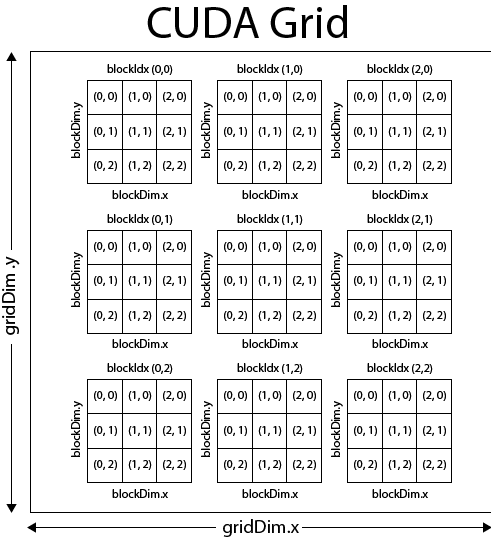
\includegraphics[width=0.5\textwidth]{imagens/gridblock_thread.png}
  \caption{Esquema de identificação de threads e blocos em CUDA. \cite{mckennon:2013}}
  \label{fig:gridblock_thread}
\end{figure}

\subsection{Stencil} \label{subsec:stencil}
O stencil é amplamente usado em várias aplicações que utilizam a ciência computacional, como  geofísica, astrofísica, física nuclear  ou oceanográfica. Estas ciências necessitam de uma larga simulação computacional com uma frequência muito alta de saída. Quando é utilizado equações diferenciais parciais (EDP) normalmente elas são resolvidas pelo método das diferenças finitas, de modo a utilizar os stencil para calcular os operadores diferenciais representando uma grande fração do tempo total de execução.

Quando se está usando o stencil, para cada ponto, por exemplo de uma matriz 2D, é usado o peso dos pontos vizinhos, assim resolvendo os operadores diferenciais espacialmente, como mostra a Figura~\ref{fig:stencil_2d}. Desta forma, replicando as operações para todos os pontos do conjunto, que ao intuito de agilizar os cálculos, pode ser feito uma paralelização entre todos os pontos de modo ideal, fazendo com que cada \emph{thread} um ponto para calcular, assim, possibilitando a paralelização do código. \cite{cruz:2015}

\begin{figure}[ht]
  \centering
  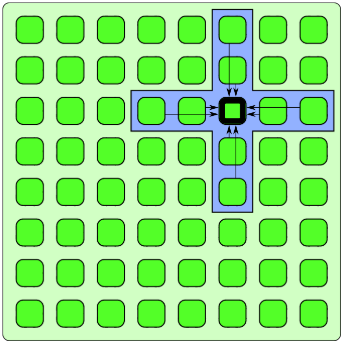
\includegraphics[width=0.3\textwidth]{imagens/stencil_2d-teoric.png}
  \caption{Exemplo de stencil 2D. \cite{phdthesis:2018}}
  \label{fig:stencil_2d}
\end{figure}

\subsection{GPU} \label{subsec:gpu}
A Unidade de Processamento Gráfico (\emph{Graphics Processing Unit}, GPU) é um Processador especializado para o aceleramento do processamento gráfico, especialmente em aplicações como renderização 3D, além do processamento de imagens. Com o avanço da arquiteturas computacionais, as GPUs evoluíram para plataformas de computação paralela de propósito geral, amplamente utilizadas em ciência de dados, aprendizado de máquina, simulações físicas e outras aplicações de alta performance, conhecidas como \emph{General-Purpose Graphics Processing Unit} (GPGPU). \cite{owens:2008}

Enquanto que as CPUs são otimizadas para a latência, uma GPU é otimizada para várias threads simultaneamente, dado a sua arquitetura massivamente paralela. Isso se dá ao fato de que a GPU é composta por centenas ou milhares de núcleos simplesmente organizados em múltiplos blocos, chamados \emph{Streaming Multiprocessors} (SMs). Cada SM é projetado para executar centenas de threads em paralelo, com um modelo de execução baseado em \emph{Single Instruction, Multiple Thread} (SIMT), uma das classificações de Flynn.

\subsubsection{GPU T4} \label{subsubsec:gpu_t4}
As GPUs T4 são baseadas na arquitetura Turing da NVIDIA, representam um avanço significativo no uso de GPUs para computação de propósito geral e aprendizado de máquina. A T4 foi projetada para ser uma solução otimizada para data centers modernos, suportando cargas de trabalho mistas que incluem treinamento, inferência, virtualização e serviços baseados em IA.

A GPU T4 tem uma memória compartilhada de 49KB, 4 MB de memória cache L2, Warp Size de 32 threads (Quantidade de threads que podem ser usadas simultaneamente). Os máximo de threads por bloco e multiprocessador é de 1024 e são 40 multiprocessadores, com uma dimensão máxima (1024, 1024, 64) de threads por bloco, em (x, y, z), já o grid é de (2147483647, 65535, 65535).

A Figura~\ref{fig:archT4} representa o esquemático da configuração da arquitetura da NVIDIA Tesla T4.

\begin{figure}[ht]
  \centering
  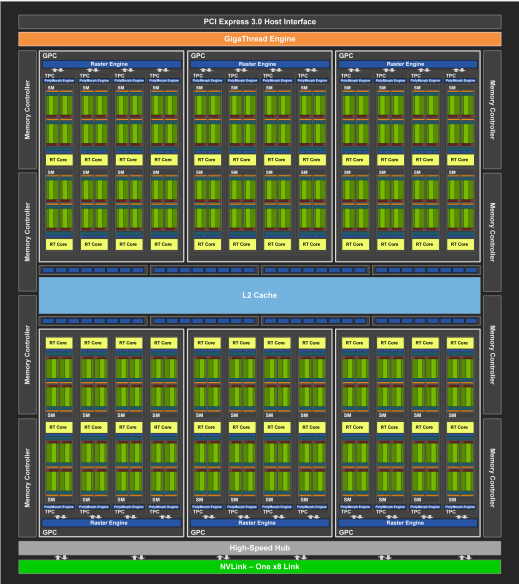
\includegraphics[width=0.6\textwidth]{imagens/gpu-t4.png}
  \caption{Arquitetura da GPU Testa T4. \cite{nvidia:2018}}
  \label{fig:archT4}
\end{figure}



% Seção de Desenvolvimento
\section{Desenvolvimento} \label{sec:desenvolvimento}

A simulação de um modelo de difusão de contaminantes em água pode ser equacionado por:

\[
\frac{\partial C}{\partial t} + \mathbf{v} \cdot \nabla C = D \nabla^2 C
\]

Onde:
\begin{itemize}
    \item \( C \) é a concentração do contaminante.
    \item \( t \) é o tempo (em segundos).
    \item \( \mathbf{v} \) é o vetor de velocidade do fluxo da água.
    \item \( D \) é o coeficiente de difusão do contaminante na água.
    \item \( \nabla^2 C \) é a ataxa de variação da concentração no espaço.
\end{itemize}

Ou ainda, pode ser formulada de uma modo mais extenso

\[
C^{(t+1)}_{i,j} = C^{(t)}_{i,j} + D \cdot \Delta t \cdot \frac{C^{(t)}_{i+1,j} + C^{(t)}_{i-1,j} + C^{(t)}_{i,j+1} + C^{(t)}_{i,j-1} - 4 \cdot C^{(t)}_{i,j}}{\Delta x^2}
\]

\subsection{Paralelizando com o CUDA: Stencil 1D}
\label{desenv:stencil1d}
O stencil 1D utiliza um vetor unidirecional para realizar os cálculos, tendo o cuidado de não acessar espaços de memória que não possam ser acessados.

\vspace{0.5cm}
\begin{lstlisting}[language=C, caption={Chamada do \emph{kernel}.}, label={lst:diff_eq}]
double diff_eq(double *C, double *C_new) {
    double *d_C, *d_C_new;
    double *swap;


    cudaMalloc( (void **) &d_C, SIZE);
    cudaMalloc( (void **) &d_C_new, SIZE);


    cudaMemcpy(d_C, C, SIZE, cudaMemcpyHostToDevice );
    cudaMemcpy(d_C_new, C_new, SIZE, cudaMemcpyHostToDevice );


    double difmedio;


    for (int t = 0; t < T; t++) {
        diff_eq_kernel<<< (N * N + (THREADS_PER_BLOCK-1)) / THREADS_PER_BLOCK, THREADS_PER_BLOCK >>>(d_C, d_C_new, N);


        cudaDeviceSynchronize();


        swap = d_C;
        d_C = d_C_new;
        d_C_new = swap;


        if (t%100==0) {
            difmedio = .0;
            cudaMemcpy(C, d_C, SIZE, cudaMemcpyDeviceToHost);
            cudaMemcpy(C_new, d_C_new, SIZE, cudaMemcpyDeviceToHost);


            for(int i=0; i<N*N; i++)
                difmedio += fabs(C[i] - C_new[i]);


            printf("interacao %d - diferenca=%g\n", t, difmedio/((N-2)*(N-2)));
        }
    }


    cudaMemcpy(C, d_C, SIZE, cudaMemcpyDeviceToHost);


    cudaFree(d_C);
    cudaFree(d_C_new);


    return C[(N/2) * N + (N/2)];
}
\end{lstlisting}
\vspace{0.5cm}

No trecho de código mostrado na Figura acima, é onde ocorre o preparo das variáveis para entrar no kernel, com as funções do cuda, como \texttt{cudaMalloc} e \texttt{cudaMemcpy}. As variáveis chaves são \texttt{d\_C}, que contém a concentração atual, \texttt{d\_C\_new}, que calcula a próxima concentração da água, \texttt{swap}, uma variável auxiliar para troca entre o \texttt{d\_C} e \texttt{d\_C\_new}. Ainda há a variável \texttt{difmedio}, para calcular a concentração média.

\'E chamado a fun\c{c}\~ao do kernel, \texttt{diff\_eq\_kernel}, passando os par\^ametros da quantidade de threads e a quantidade de blocos, al\'em das vari\'aveis para o c\'alculo da concentra\c{c}\~ao e a dimens\~ao da grade, dado que ela \'e um quadrado.

Após a chamada é feita a sincronização com os threads e a troca de ponteiros pela variável. Também é mostrado a concentração média quando a iteração é múltipla de 100, passando os resultados para as variáveis do Host.

Quando todas as interações acabarem, as variáveis do device são liberadas e a concentração do meio é retornada. 

\vspace{0.5cm}
\begin{lstlisting}[language=C, caption={}, label={}]
__global__ void diff_eq_kernel(double *C, double *C_new, int n) {
    int in  dex = threadIdx.x + blockIdx.x * blockDim.x;


    if (index >= n && index < n * (n - 1) && index % n != 0 && index % n != n - 1) {
        C_new[index] = C[index] + D * DELTA_T * (
            (C[index+1] + C[index-1] + C[index+N] + C[index-N] - 4*C[index]) / (DELTA_X * DELTA_X)
        );
    }
}
\end{lstlisting}
\vspace{0.5cm}

A Figura acima mostra a funcionalidade da função do kernel, que calcula a próxima concentração, utilizando apenas vetores unidirecionais, mas que representam a matriz, apenas estão agrupadas em uma única dimensão. Note que é calculado o índice da thread que fará o cálculo. Observe que as bordas da matriz não são calculadas, ou seja, o lado esquerdo não tem relação alguma com o lado direito, ou em cima não tem relação com a parte de baixo. Já a equação é a mesma utilizada no código sequencial.


\subsection{Paralelizando com o CUDA: Stencil 2D}
\label{desenv:stencil2d}
O stencil 2D já utiliza uma matriz para realizar os cálculos, também com o cuidado de não acessar espaços de memória que não possam ser acessados. Contudo, a diferença entre o stencil 1D e o 2D é que, nessa implementação, no stencil 2D utilizou-se duas dimensões para encontrar o índice da \emph{thread}. Especificamente as dimensões x e y da matriz do grid.

A implementação da chamada do \emph{kernel} é bem similar à do stencil 1D, com pequenas variações entre as implementações, já que todos os laços percorrerão em outro laço, formando assim uma complexidade maior de cálculos. A implementação e chamada do \emph{kernel} pode ser vista na Listagem~\ref{lst:diff_eq_2d}.

\vspace{0.5cm}
\begin{lstlisting}[language=C, caption={Função principal com a chamada do \emph{kernel} 2D.}, label={lst:diff_eq_2d}]
int main() {
    double *C, *C_new;
    double *d_C, *d_C_new;
    size_t size = MEM_SIZE_MATRIX;

    // Alocar memoria no host
    C = (double*)malloc(size);
    C_new = (double*)malloc(size);

    if (C == NULL || C_new == NULL) {
        fprintf(stderr, "Memory allocation failed\n");
        return 1;
    }

    // Inicializar matrizes
    initialize_matrix(C, N);
    initialize_matrix(C_new, N);

    // Alocar memoria na GPU
    check_cuda_error(
        cudaMalloc((void**)&d_C, size), "Failed to allocate device memory for C");
    check_cuda_error(
        cudaMalloc((void**)&d_C_new, size), "Failed to allocate device memory for C_new");

    // Copiar dados do host para a GPU
    check_cuda_error(
        cudaMemcpy(d_C, C, size, cudaMemcpyHostToDevice), "Failed to copy data from host to device");

    // Configurar grade e blocos
    dim3 block(BLOCK_SIZE_X, BLOCK_SIZE_Y);
    dim3 grid((N + block.x - 1) / block.x, (N + block.y - 1) / block.y);

    double difmedio;

    // Calculando o tempo de execucao
    double iStart = omp_get_wtime();

    // Executar kernel
    for (int t = 0; t < T; t++) {
        diff_eq_kernel<<<grid, block>>>(d_C, d_C_new, N);
        check_cuda_error(
            cudaDeviceSynchronize(), "Kernel execution failed");

        // Trocar ponteiros
        double *swapAux = d_C;
        d_C = d_C_new;
        d_C_new = swapAux;

        if (t % 100 == 0) {
            difmedio = 0.0;
            check_cuda_error(
                cudaMemcpy(C, d_C, size, cudaMemcpyDeviceToHost), "Failed to copy data from device to host");
            check_cuda_error(
                cudaMemcpy(C_new, d_C_new, size, cudaMemcpyDeviceToHost), "Failed to copy data from device to host");

            for (int i = 0; i < N * N; i++)
                difmedio += fabs(C[i] - C_new[i]);

            printf("interacao %d - diferenca=%g\n", t, difmedio / ((N - 2) * (N - 2)));
        }
    }

    double iElaps = omp_get_wtime() - iStart;

    // Metricas
    printf("\n<<<%d,%d>>>;");
    printf("%lf\n", iElaps);

    // Copiar resultado de volta para o host
    check_cuda_error(
        cudaMemcpy(C, d_C, size, cudaMemcpyDeviceToHost), "Failed to copy data from device to host");

    // Liberar memoria na GPU
    cudaFree(d_C);
    cudaFree(d_C_new);

    // Liberar memoria no host
    free(C);
    free(C_new);

    return 0;
}
\end{lstlisting}
\vspace{0.5cm}

Diante da Listagem~\ref{lst:diff_eq_2d}, observa-se que, inicialmente, são alocados os ponteiros responsáveis por armazenar os valores das matrizes. Destaca-se a chamada da função \texttt{initialize\_matrix}, que realiza a alocação de memória para as estruturas e inicializa o valor no centro da matriz \texttt{C}. Em seguida, a memória é alocada na GPU utilizando a função \texttt{cudaMalloc}, e os dados são transferidos do host para a GPU por meio da função \texttt{cudaMemcpy}.

Após essa etapa, configura-se a grade e os blocos utilizando a função \texttt{dim3}, uma estrutura que define as dimensões da grade e dos blocos. Por fim, um laço de repetição é executado para \texttt{T} iterações, em que o \emph{kernel} \texttt{diff\_eq\_kernel} é invocado para calcular a difusão do contaminante na água. Em cada iteração, a concentração é calculada com base na técnica de programação Stencil. Ao término do laço, os dados são copiados da GPU para o host, e a memória alocada tanto na GPU quanto no host é liberada.

A Listagem~\ref{lst:diff_eq_kernel_2d} mostra a implementação do \emph{kernel} que realiza os cálculos e também verifica os índices úteis para o stencil, já que deve-se descontar o raio do stencil para não acessar posições inválidas da matriz. Em contraste com o \emph{kernel}, as Listagens \ref{lst:initialize_matrix} e \ref{lst:check_cuda_error} mostram as funções utilizadas para alocar e inicializar as matrizes e para verificar os erros de execução do CUDA, respectivamente.

\vspace{0.5cm}
\begin{lstlisting}[language=C, caption={\emph{Kernel} 2D.}, label={lst:diff_eq_kernel_2d}]
__global__ void diff_eq_kernel(double *C, double *C_new, int n) {
    int x = blockIdx.x * blockDim.x + threadIdx.x;
    int y = blockIdx.y * blockDim.y + threadIdx.y;
    int index = y * n + x;

    if (x > 0 && x < n - 1 && y > 0 && y < n - 1) {
        C_new[index] = C[index] + D * DELTA_T * (
            (C[index + 1] + C[index - 1] + C[index + n] + C[index - n] - 4 * C[index]) / (DELTA_X * DELTA_X)
        );
    }
}
\end{lstlisting}

\begin{lstlisting}[language=C, caption={Inicialização e alocação das matrizes.}, label={lst:initialize_matrix}]
void initialize_matrix(double *m, int n) {
    for (int i = 0; i < n; i++) {
        for (int j = 0; j < n; j++) {
            m[i * n + j] = 0.0;
        }
    }
    m[(n / 2) * n + (n / 2)] = 1.0;
}
\end{lstlisting}

\begin{lstlisting}[language=C, caption={Verificação de erros do CUDA.}, label={lst:check_cuda_error}]
void check_cuda_error(cudaError_t err, const char *msg) {
    if (err != cudaSuccess) {
        fprintf(stderr, "CUDA Error: %s: %s\n", msg, cudaGetErrorString(err));
        exit(EXIT_FAILURE);
    }
}
\end{lstlisting}
\vspace{0.5cm}

Observe que, diferentemente do \emph{Stencil} 1D desenvolvido no subcapítulo \ref{desenv:stencil1d}, o \emph{kernel} criado para o \emph{Stencil} 2D possui índices em função de duas dimensões, calculados a partir dos métodos \texttt{blockIdx.x}, \texttt{blockDim.x} e \texttt{threadIdx.x}, assim como dos métodos aplicados na dimensão \texttt{y}.


% Seção de Resultados
\section{Resultados} \label{sec:resultado}
Após as implementações realizadas e mostradas na seção \ref{sec:desenvolvimento}, foram realizados testes de desempenho para avaliar a eficácia da paralelização do modelo criado. As Figuras~\ref{fig:grafico_resultados-stencil2D} e \ref{fig:grafico_resultados-stencil1D} mostram os resultados obtidos para o \emph{Stencil} 2D e 1D, respectivamente.

\begin{figure}[ht]
    \centering
    
\includegraphics[width=0.8\textwidth]{imagens/grafico_resultados-stencil2D.png}
    \caption{Gráfico de desempenho do \emph{Stencil} 2D.}
    \label{fig:grafico_resultados-stencil2D}
\end{figure}

Diante os resultados das Figuras \ref{fig:grafico_resultados-stencil2D} e \ref{fig:grafico_resultados-stencil1D}, pode-se verificar que os resultados para diversas configurações de \emph{grids} e \emph{blocks} foram satisfatórios, já que para um problema com um número expressivo de iterações, o tempo de processamento total está na ordem de milissegundos. Contudo, é possível observar que o \emph{Stencil} 2D obteve um desempenho superior ao \emph{Stencil} 1D, o que pode ser justificado pela complexidade do cálculo, que envolve mais operações matriciais. Ainda sobre os resultados do \emph{stencil} 2D, também pode-se observar que a configuração em que o número de blocos e o número de \emph{threads} por bloco são de 7875 e 512, respectivamente.

\begin{figure}[ht]
    \centering
    
\includegraphics[width=0.8\textwidth]{imagens/grafico_resultados-stencil1D.png}
    \caption{Gráfico de desempenho do \emph{Stencil} 1D.}
    \label{fig:grafico_resultados-stencil1D}
\end{figure}

Já sobre o \emph{stencil} 1D, o desempenho também foi satisfatório mas inferior ao \emph{stencil} 2D, o que pode ser explicado pela forma como os dados são acessados na memória. A configuração que apresentou melhor desempenho foi com 16384 blocos e 256 \emph{threads} por bloco (64 \emph{threads} por bloco), resultando em um tempo de execução médio de 281 milissegundos.

Comparando as duas implementações, pode-se observar que ambas as abordagens atingiram resultados expressivos em termos de desempenho. O \emph{stencil} 2D demonstrou ser mais eficiente para este problema específico, possivelmente devido à melhor utilização da localidade espacial da memória e ao padrão de acesso aos dados mais otimizado. Por outro lado, o \emph{stencil} 1D, embora com tempos de execução ligeiramente superiores, ainda manteve um excelente desempenho, demonstrando que ambas as estratégias são viáveis para a resolução do problema.

A Tabela \ref{tab:comparacao_implementacoes} apresenta uma comparação entre as melhores médias das amostras quando implementadas em código sequencial, OpenMP e CUDA. Deve-se levar em consideração a confiabilidade dos resultados, já que o número de testes realizados foi superior a 30. Diante os resultados obtidos, a implementação que melhor performou foi a codificação utilizando a tecnologia CUDA, com um \emph{speedup} de 80.1603 em relação à implementação sequencial. Por fim, a eficiência da implementação em CUDA não foi calculada, já que a modelagem CUDA apresenta características únicas, quando comparadas às demais. Portanto, o cálculo da eficiência para tal arquitetura deve ser diferente e não foi considerado para esse trabalho. 

\begin{table}[ht]
    \centering
    \caption{Comparação entre as diferentes implementações}
    \begin{tabular}{|c|c|c|c|}
        \hline
        \textbf{Implementação} & \textbf{Tempo (ms)} & \textbf{Speedup} & \textbf{Eficiência} \\
        \hline
        Sequencial & 21.507 & 1.00 & 1.00 \\
        \hline
        OpenMP & 16.1707 & 1.3300 & 0.3325 \\
        \hline
        CUDA 1D & 0.2810 & 76.5374 & - \\
        \hline
        CUDA 2D & 0.2683 & 80.1603 & - \\
        \hline
    \end{tabular}
    \label{tab:comparacao_implementacoes}
\end{table}

% Seção da conclusão
\section{Conclusão} \label{sec:conclusao}
Os resultados obtidos demonstram que a paralelização em GPU utilizando CUDA foi extremamente bem-sucedida, reduzindo significativamente o tempo de processamento em comparação com uma possível implementação sequencial. Além disso, as diferentes configurações de blocos e \emph{threads} testadas permitiram identificar as combinações ideais para cada implementação, otimizando ainda mais o desempenho do algoritmo.

Este trabalho apresentou a implementação e análise de diferentes abordagens para a simulação da difusão de contaminantes em água, utilizando técnicas de programação paralela em CPU (OpenMP) e GPU (CUDA). Os resultados obtidos demonstraram que a paralelização em GPU utilizando CUDA foi extremamente bem-sucedida, alcançando um speedup de até 80.1603 vezes em relação à implementação sequencial.

A comparação entre as implementações 1D e 2D em CUDA revelou que ambas as abordagens são eficientes, com a implementação 2D apresentando um desempenho ligeiramente superior. Esta diferença pode ser atribuída à melhor utilização da localidade espacial da memória e ao padrão de acesso aos dados mais otimizado na versão 2D.

Por fim, é importante ressaltar que a implementação OpenMP, embora tenha apresentado uma melhoria de desempenho mais modesta (speedup de 1.33), também contribuiu para a redução do tempo de processamento. No entanto, a tecnologia CUDA demonstrou ser a escolha mais adequada para este tipo de problema, devido à sua capacidade de explorar o alto grau de paralelismo oferecido pelas GPUs.


% Seção das referências
\section{Referências} \label{sec:referencias}
\bibliographystyle{sbc}
\bibliography{sbc-template}


\end{document}